\documentclass{standalone}
%-----------------------------------------------------------------------------%
%%% Math %%%
\usepackage{amsmath,mathtools,amssymb,mathrsfs}
%-----------------------------------------------------------------------------%
%%% Probability %%%
\let\Pr\relax
\DeclareMathOperator{\Pr}{\text{\upshape\textbf{P}}}
%-----------------------------------------------------------------------------%
%%% TikZ %%%
\usepackage{tikz}
%-----------------------------------------------------------------------------%

\begin{document}

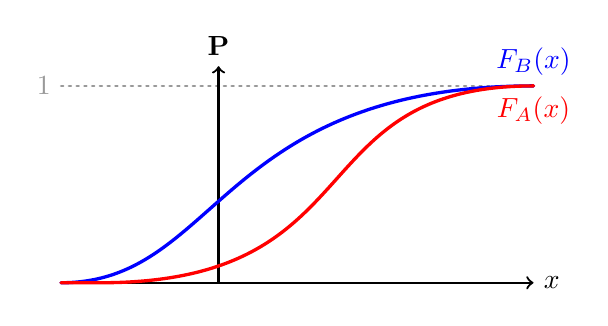
\begin{tikzpicture}[thick,line cap=round,yscale=5,scale=0.5]
	%% 1
	\draw[dotted,opacity=0.4] (-4,1) node[left]{$1$} -- (8,1);
	%% Axis
	\draw[->] (-4,0) -- (8,0) node[right]{$x$};
	\draw[->] (0,0) -- (0,1.1) node[above]{$\Pr$};
	%% CDF
	\draw[very thick,blue]  (-4,0) .. controls (0,0) and (0,1) .. (8,1) node[above]{$F_B(x)$};
	\draw[very thick,red] (-4,0) -- (-3,0) .. controls (4,0) and (2,1) .. (8,1) node[below]{$F_A(x)$};
\end{tikzpicture}

\end{document}
